%%%%%%%%%%%%%%%%%%%%%%%%%%%%%%%%%%%%%%%%%%%%%%%%%%%%%%%%%%%%%%%%%%%%%%%
% Sample template for MIT Junior Lab Student Written Summaries
% Available from http://web.mit.edu/8.13/samplepaper/sample-paper.tex
%
% Last Updated June 20, 2004
%
% Adapted from the American Physical Societies REVTeK-4 Pages
% at http://publish.aps.org
%
% ADVICE TO STUDENTS: Each time you write a paper, start with this
%    template and save under a new filename.  If convenient, don't
%    erase unneeded lines, just comment them out.  Often, they
%    will be useful containers for information.
%%%%%%%%%%%%%%%%%%%%%%%%%%%%%%%%%%%%%%%%%%%%%%%%%%%%%%%%%%%%%%%%%%%%%%%


%%%%%%%%%%%%%%%%%%%%%%%%%%%%%%%%%%%%%%%%%%%%%%%%%%%%%%%%%%%%%%%%%%%%%%%
% PREAMBLE
% The preamble of a LaTeX document is the set of commands that precede
% the \begin{document} line.  It contains a \documentclass line
% to load the REVTeK-4 macro definitions and various \usepackage
% lines to load other macro packages.
%
% ADVICE TO STUDENTS: This preamble contains a suggested set of
%     class options to generate a ``Junior Lab'' look and feel that
%     facilitate quick review and feedback from one's peers, TA's
%     and section instructors.  Don't make substantial changes without
%     first consulting your section instructor.
%%%%%%%%%%%%%%%%%%%%%%%%%%%%%%%%%%%%%%%%%%%%%%%%%%%%%%%%%%%%%%%%%%%%%%%

\documentclass[aps,twocolumn,secnumarabic,nobalancelastpage,amsmath,amssymb,
nofootinbib]{revtex4}

% nofootinbib is another document class option that allows you to put
% footnotes on the page where they occur rather than at the end of the
% paper.  This makes for easier reading!

% secnumarabic is a particularly nice way of identifying sections by
% number to aid electronic review and commentary.

% amsmath and amssymb are necessary for the subequations environment
% among others

\usepackage{graphics}      % standard graphics specifications
\usepackage{graphicx}      % alternative graphics specifications
\usepackage{longtable}     % helps with long table options
\usepackage{url}           % for on-line citations
\usepackage{bm}            % special 'bold-math' package
\usepackage{subfigure}
\usepackage{booktabs}

%%%%%%%%%%%%%%%%%%%%%%%%%%%%%%%%%%%%%%%
%                                 %%%%%
% And now, begin the document...  %%%%%
%                                 %%%%%
%%%%%%%%%%%%%%%%%%%%%%%%%%%%%%%%%%%%%%%
\begin{document}
\title{Rutherford Scattering}
\author         {Kevin L. Chen. Partner: Tanooj Shah}
\affiliation    {UC Berkeley, Department of Physics}
\date{\today}

\begin{abstract}
% Do at the end
\end{abstract}

\maketitle

%%%%%%%%%%%%%%%%%%%%%%%%%%%%%%%%%%%%%%%%%%%%%%%%%%%%%%%%%%%%%%%%%%%%%%%%%%%%%
\section{Introduction}

Atomic Spectroscopy is one of the fundamental fields of physics where Quantum Mechanics its energy level became more robust theoretically. From atomic spectroscopy, physicists have discovered the Rydberg Formula, illustrating the transitions between electron energy levels. One of the most important of these transitions are called the Balmer Series, which depicts the transitions from n > 3 states to n = 2 stages. The light from this series is visible light. Furthermore, by introducing a magnetic field to the atom, we add a new term to the Hamiltonian. This new term gives rise to Zeeman splitting. With this magnetic field, we see spectral lines splitting, due to a split in the energy levels. Using modern day optics and spectroscopic techniques, we can use these spectral lines to determine the Rydberg Constant and the Bohr Magneton. 
%%%%%%%%%%%%%%%%%%%%%%%%%%%%%%%%%%%%%%%%%%%%%%%%%%%%%%%%%%%%%%%%%%%%%%%%%%%%%
\section{Theory}
\subsection{Balmer Series}

To begin speaking about the Balmer Series, one must understand the Bohr Model. In this mode of an atom, the electron revolves around the nucleus of the atom, much like a planet revolves around the sun. Therefore, we have a force balance equation 

\begin{equation}
    {m_\mathrm{e} v^2\over r} = {Zk_\mathrm{e} e^2 \over r^2} 
   \label{Bohr Model}
\end{equation}

where $m_e$ is the electron's mass, $e$ is the charge of the electron, $k_e$ is Coulomb's constant and $Z$ is the atom's atomic number. However, unlike in classical mechanics where the angular momentum is continuous, quantum mechanics exhibits discrete values of angular momentum. Specifically, the angular momentum is an integer multiple of Planck's Constant:

\begin{equation}
     m_\mathrm{e} v r = n \hbar 
   \label{Quantized L}
\end{equation}

where $n$ is the Principle Quantum Number. 

By combining Equation~\ref{Bohr Model} and Equation~\ref{Quantized L}, we arrive at the relationship between the Principle Quantum number and the corresponding energy:

\begin{equation}
      E = - { Z^2(k_\mathrm{e} e^2)^2 m_\mathrm{e} \over 2\hbar^2 n^2} \approx {-13.6Z^2 \over n^2}\mathrm{eV}
   \label{Energy Level for nth Level}
\end{equation} 

The Balmer Series are the series of transitions where atoms end up in the $n = 2$ state. This means any transition from $n > 2$ to $n = 2$ is a Balmer Series transition. These transitions result in energy loss in the form of a photon, which is what we observed as visible spectrum lines. The energies of these photons are described by this energy difference relation, called the Rydberg Formula:

\begin{equation} 
    E=E_i-E_f=R_\mathrm{E} \left( \frac{1}{n_{f}^2} - \frac{1}{n_{i}^2} \right) \,
  \label{Rydberg Forumla}
\end{equation}

and since $ E = hc / \lambda $, the above equation can be rewritten as 

\begin{equation} 
    \frac{1}{\lambda}=R \left( \frac{1}{n_{f}^2} - \frac{1}{n_{i}^2} \right). \,
  \label{Use this Rydberg Formula}
\end{equation}

where $n_{f} = 2$ for the Balmer Series.

In this experiment, we use Equation~\ref{Use this Rydberg Formula} to determine the Rydberg Constant, $R$, by plotting $1 / \lambda$ against $1 / n^{2} $.

\subsection{Zeeman Effect}

Another quantum effect we observe in this experiment is the Zeeman Effect, where a weak magnetic field is applied to atoms, adding a term to their Hamiltonian, and thus splitting energy levels. 

We begin with the Hamiltonian of an atom: 

\begin{equation}
    H = H_0 -\vec{\mu} \cdot \vec{B}, \: \: \vec\mu =\frac{e}{2m_e}g\vec j
  \label{Hamiltonian}
\end{equation}

where $H_0$ is the unperturbed Hamiltonian and the second term is the term resulting from the Zeeman Effect. The other terms $\vec\mu$ are as follows: 

\begin{itemize}
 \item $e$ is the fundamental charge value
 \item $m_e$ is the mass of the electron
 \item $\vec B$ is the magnetic field
 \item $\vec j$ is the total angular momentum resulting from a sum of the electron's orbital angular momentum $\vec l$ and its spin angular momentum $\vec s$
 \item $g$ is the Lande-g Factor (a multiplicative factor that arises when a weak magnetic field is introduced to the atom.) given by:

\begin{equation}
  g_J \approx \frac{3}{2}+\frac{S(S+1)-L(L+1)}{2J(J+1)}. 
  \label{Lande G}
\end{equation}

\end{itemize}

By taking the dot product, we get the projection of the angular momentum $\vec j$ against the axis of the magnetic field, which results in the following energy perturbation:

\begin{equation} 
  \Delta E = \mu_0 B \Delta (g m_j)
  \label{Zeeman Energies}
\end{equation}

This $m_j$ terms are what the energy levels split into, and can take on the integral values from $-j$ to $+j$ depending on the j value. 

\begin{figure}[t]
  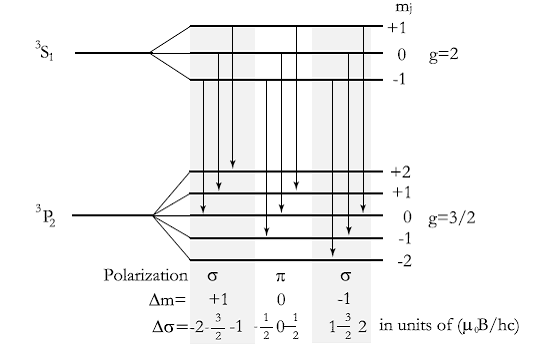
\includegraphics[width = 0.4\textwidth]{ZeemanSplitting.png}
  \begin{center}
  \caption{Structure of the Zeeman multiplet arising in a transition from a $^{3}S_1$ to a $^{3}P_2$ level.}[\footnotesize{``Atomic Physics.'' - Physics 111-Lab Wiki. UC Berkeley, n.d. Web. 23 Apr. 2015.}]
  \label{ZeemanSplitting}
  \end{center}
\end{figure}

An important part of this experiment is the Fabry -- P\'{e}rot interferometer, which is discussed in depth in Section~\ref{FPI}. A relation that arises from this device is the Free Spectral Range, which relates the wave number to the properties of the F--P interferometer. 

\begin{equation} 
  \Delta \sigma = \frac{\alpha}{2tn}
  \label{FP Equation}
\end{equation}

where $\alpha$ is a constant depending on how much Zeeman Splitting we induce, $n$ is the index of refraction of air, $t$ is the thickness of the interferometer, and $\sigma$ is the wave number. We also know through the deBroglie relations that 

\begin{equation}
  E = hc/\lambda 
  \label{deBroglie}
\end{equation}

and since $\lambda = 1 / \sigma$, then $E = hc\sigma$ and $\Delta E = hc \Delta \sigma$. A change in energy from Equation~\ref{Zeeman Energies} results in $\Delta E = \mu_0 B \Delta (m_j g)$. Relating this to Equation~\ref{FP Equation} and Equation~\ref{Zeeman Energies}, we get the relationship to find the Bohr Magneton:

\begin{equation}
  \mu_0 = \frac{h c \alpha}{2 t n B \Delta(g m_j)}
  \label{Bohr Magneton}
\end{equation}

\subsection{Broadening}

\begin{figure}[t]
  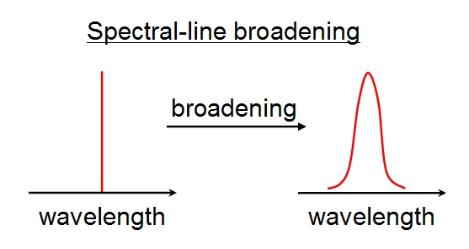
\includegraphics[width = 5 cm]{Broadening.jpg}
  \begin{center}
  \caption{Broadening, caused by several factors like natural broadening, thermal broadening, and collision broadening.}[\footnotesize{``CV Accretion Discs." CV Accretion Discs. N.p., n.d. Web. 24 Apr. 2015.}]
  \label{Broadening}
  \end{center}
\end{figure}

If each electron transition was just to emit a photon with a well defined energy and, thus, one wavelength, then the spectral line we ought to observe would be infinitely thin (Left side of Fig~\ref{Broadening}). However, several factors give the line a width: the uncertainty principle,

\begin{equation}
   \Delta{E}\Delta{t} \geq \frac{\hbar}{2} \Rightarrow \Delta \nu = \frac{1}{2 \pi \Delta t}
  \label{Natural Equation}
\end{equation}

thermal broadening,

\begin{equation}
  \Delta \nu = \sqrt{\frac{8kT\ln 2}{mc^2}}\nu_{0}
  \label{Doppler Equation}
\end{equation}

and collision broadening

\begin{equation}
  \Delta \nu = \sqrt{\frac{8kT}{m}} n \sigma
  \label{Collision Equation}
\end{equation}  

Natural broadening is naturally caused by the Heisenberg Uncertainty Principle. Second, thermal Broadening is caused by the movement of the atoms. Since the gases that are being excited are moving, some atoms will be moving towards the observer, and thus emitting blue shifted light, while some atoms will move away from the observer will emit red shifted light. This frequency shifting is caused by thermal effects, and therefore is called Thermal Broadening. Last, spectral line broadening is also caused by collision broadening. If atoms that are emitting light are constantly colliding with other atoms, then their electron energy levels get spread out.

In Table~\ref{Spread}, we see that thermal broadening has the largest effect on the spread of the spectral line by almost three orders of magnitude. Since the values we used to calculate the spreads in the table are similar to the actual values in the experiment, we can assume that the largest cause in spread and uncertainty will be through thermal broadening. 

\begin{table}[h]
  \begin{tabular}{|l|l|}
  \hline
  Type of Broadening & FWHM Spread                         \\ \hline
  Natural            & 8 MHz                               \\
  Thermal            & 5 GHz                               \\
  Collision          & 13 MHz                              \\ \hline
  \end{tabular}
  \caption{The approximate spreads due to different types of broadening. Calculations were done with P $= 5$ Torr, T $= 600$ K, and $\Delta t = 10$ ns}
  \label{Spread}
\end{table}

\section{Setup}
\subsection{Balmer Series}

\begin{figure}[ht]
  \begin{center}
    \subfigure[Balmer Series Setup]{\label{Balmer}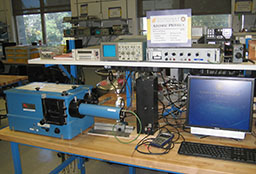
\includegraphics[width=8 cm]{BalmerSetup.jpg}}
    \subfigure[Grating in the Monochromator]{\label{Grating}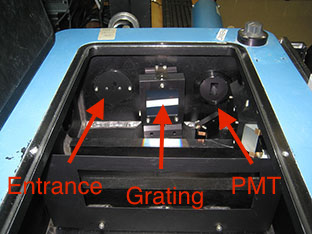
\includegraphics[width=8 cm]{Grating.jpg}} \\
  \end{center}
  \caption{Atomic Physics Experiment Setup at UC Berkeley}[\footnotesize{``Atomic Physics.'' - Physics 111-Lab Wiki. UC Berkeley, n.d. Web. 4 May. 2015.}]
  \label{ThreeFigs}
\end{figure}

\subsection{Zeeman Series}
\subsubsection{Fabry -- P\'{e}rot interferometer} \label{FPI}

\begin{figure}[t]
  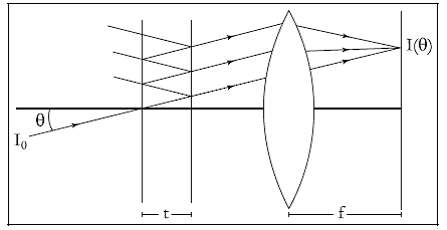
\includegraphics[width = 0.4\textwidth]{FabryPerot.png}
  \begin{center}
  \caption{A Fabry -- P\'{e}rot interferometer. The light enters the interferometer and then exists, interfering with itself and creating Airy Disks.}[\footnotesize{``Atomic Physics.'' - Physics 111-Lab Wiki. UC Berkeley, n.d. Web. 23 Apr. 2015.}]
  \label{FP}
  \end{center}
\end{figure}

A crucial piece of equipment in the Zeeman Effect portion of this experiment is the Fabry -- P\'{e}rot interferometer (Fig~\ref{FP}). This interferometer takes incoming light, reflects it multiple times within its internal mirrors, and then sends the light back out, causing the light to interfere with itself. When one observes the outgoing light from an F--P interferometer, one sees Airy Disks(Fig~\ref{AiryDisk}).

\begin{figure}[t]
  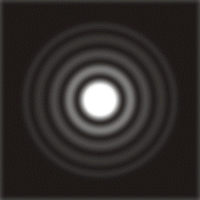
\includegraphics[width = 5 cm]{AiryDisk.png}
  \begin{center}
  \caption{An airy disk, showing interference patterns.}[\footnotesize{``Telescope Equations.": Resolving Power. N.p., n.d. Web. 23 Apr. 2015.}]
  \label{AiryDisk}
  \end{center}
\end{figure}

In this experiment, we observe a discharge tube a Helium gas. By passing the light through a red filter and then through the FP interferometer, we are able to see the Airy Disks. These disks are separated by a quantity that we will call $\Delta \sigma$, which has units of cm$^{-1}$. What is more powerful about this interferometer is that when a magnetic field is applied to the Helium gas, we see the Airy disks split, thus resembling the Zeeman splitting of the energy levels. In Fig~\ref{ZeemanSplitting}, we see that there are two different kind of transitions, $\sigma$ and $\pi$ transitions. These transitions denote the change in angular momentum. Since $m_j$ is an indicator of the angular momentum of the electron, a transition that yields a change in $m_j$ is a $\sigma$ transition and yields a change in angular momentum. $\pi$ transitions, on the other hand, do not have changes in angular momentum. 

\begin{figure}[tt]
  \begin{center}
    \subfigure[With both $\sigma$ and $\pi$ components. The top and bottom black lines are the $\sigma$ components while the middle line is the $\pi$ component.]{\label{SigmaPi}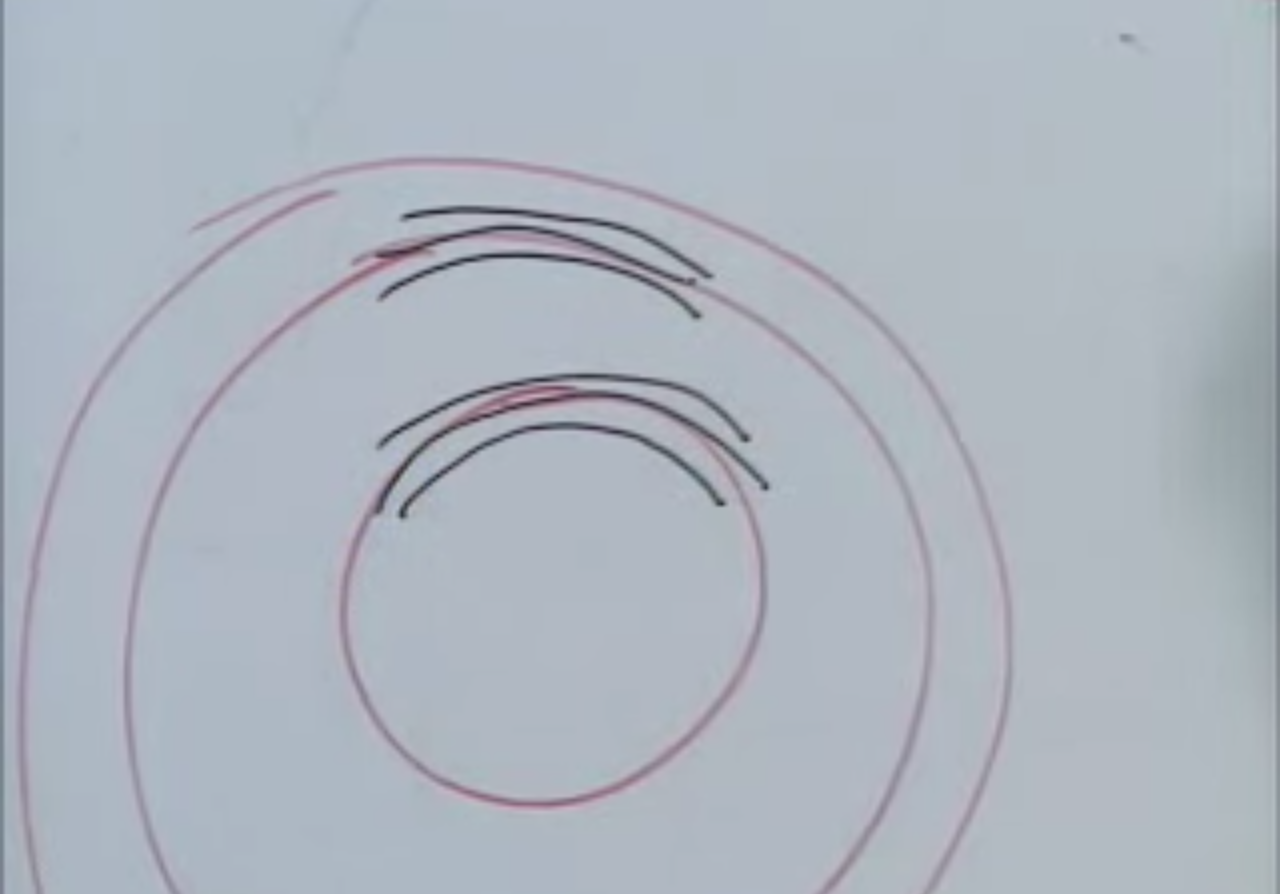
\includegraphics[width=4 cm]{sigmapi.png}}
    \subfigure[With the polarizer, eliminating the $\pi$ component.]{\label{Valve}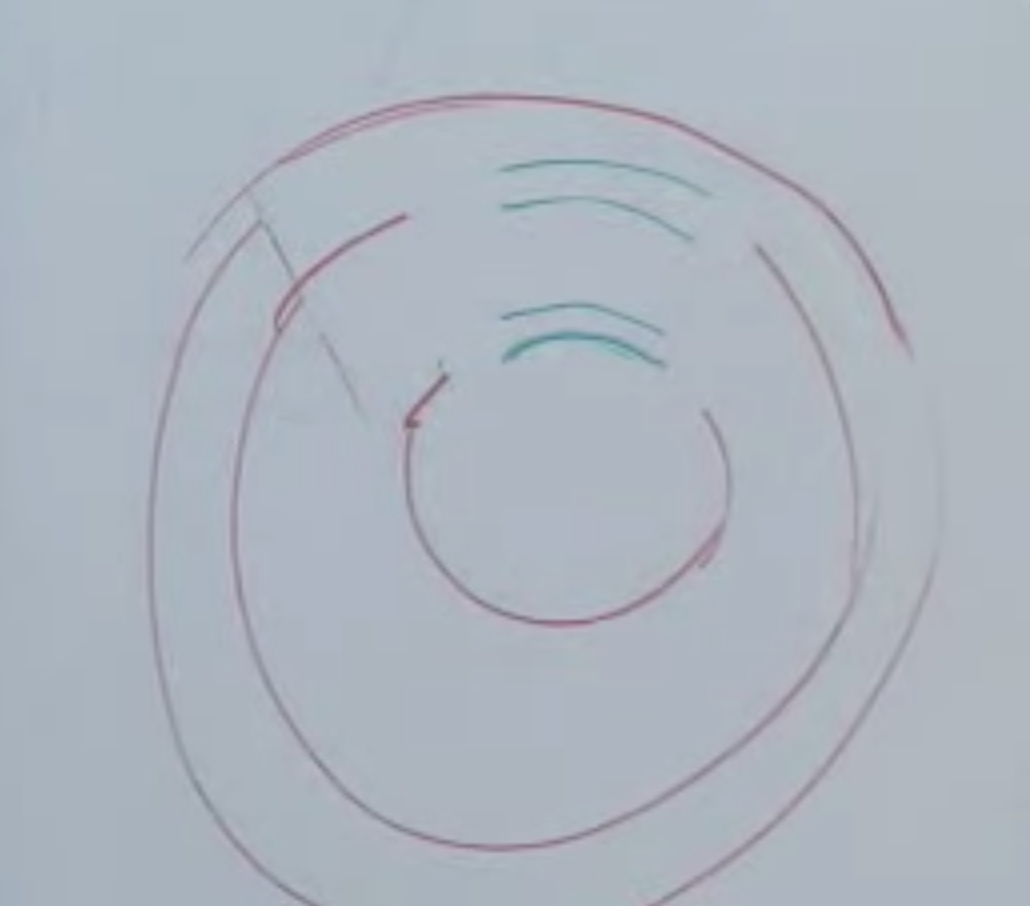
\includegraphics[width=4.3 cm]{justsigma.png}}
  \end{center}
  \caption{Zeeman Splitting showing $\sigma$ and $\pi$ Components}[\footnotesize{``Physics 111: Atomic Physics (ATM) Part 2. Zeeman Effect." YouTube. YouTube, n.d. Web. 23 Apr. 2015.}]
  \label{Sigma and Pi}
\end{figure}

We can measure these splittings independently with a polarizer. By setting the polarizer to filter out any light that is not circularly polarized, we end up seeing only the $\sigma$ transitions. Then we adjusted the magnetic field such that the airy disks were evenly spaced out. This means we had the $\sigma$ lines move $1/4 \Delta \sigma$. 

% %%%%%%%%%%%%%%%%%%%%%%%%%%%%%%%%%%%%%%%%%%%%%%%%%%%%%%%%%%%%%%%%%%%%%%%%%%%%%
% \section{Set Up}
% \subsection{Equipment}

% \begin{figure}[htp]
%   \begin{center}
%     \subfigure[Table Set-up]{\label{Table}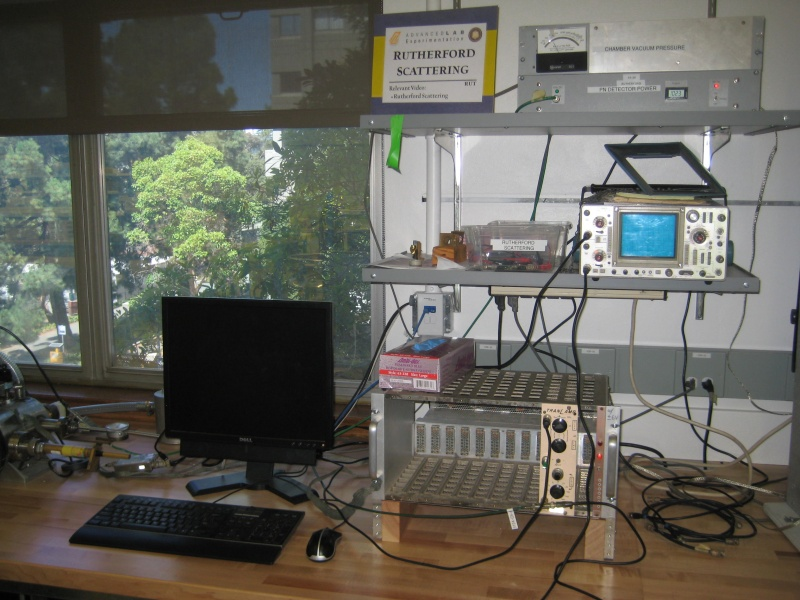
\includegraphics[width=4 cm]{RUT1.jpg}}
%     \subfigure[Vacuum Valve]{\label{Valve}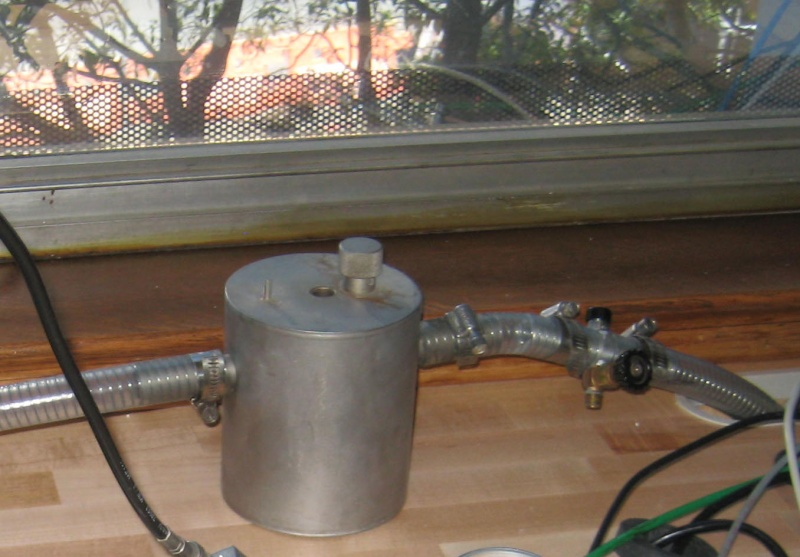
\includegraphics[width=4.3 cm]{RUT2.jpg}} \\
%     \subfigure[Scattering Chamber]{\label{Chamber}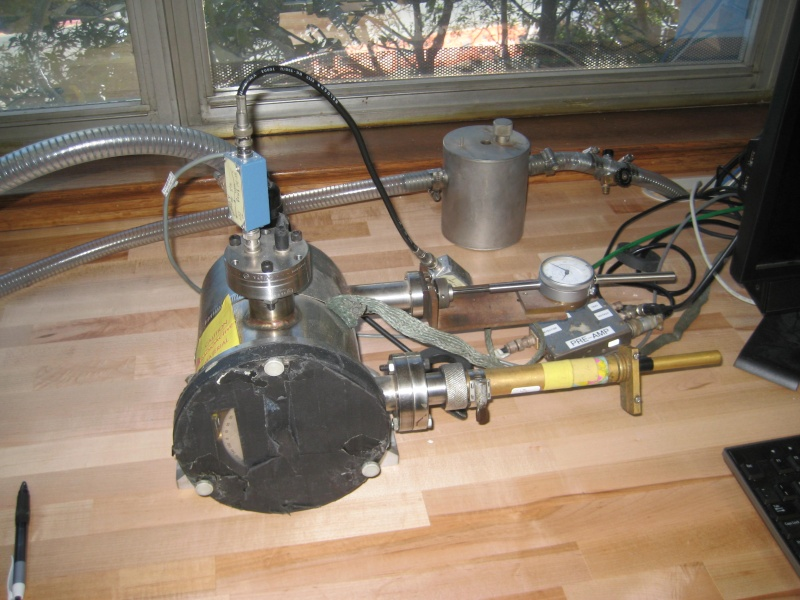
\includegraphics[width=9 cm]{RUT3.jpg}}
%   \end{center}
%   \caption{Rutherford Experiment Setup at UC Berkeley}[\footnotesize{``Rutherford Scattering.'' - Physics 111-Lab Wiki. UC Berkeley, n.d. Web. 13 Mar. 2015.}]
%   \label{ThreeFigs}
% \end{figure}

% \begin{enumerate}
% \item Vacuum Chamber with an adjustable detector and corresponding angle measure to measure the angle between the detector and the axis of the alpha gun. Our detector is a Silicon PN-junction with about 250 microns of gold on it. It has a bias of 50 volts at 4 microamps with a diameter of 0.75 inches. The detector receives its power through a voltage divider to get 50 volts from the 100 volt power supply in the rack
% \item An alpha particle source. In our experiment, we used Americium 241. 
% \item A gun in which the alpha particle is placed with an adjustable aperture size. The gun was placed 7.8 cm away from the detector. 
% \item Double layers of gold leaf foils that can be mounted in front the alpha gun.
% \item A vacuum pump.
% \item An oscilloscope to detect energy from the alpha gun. 
% \item A data taking software. In our experiment, we used a pre-coded LabVIEW program called PHA-5124. This allowed us to measure the energies, counts, and set the gain of energies of the alpha particles that interacts with the detector. 
% \item Pre-amp
% \item Tran-L-Amp
% \end{enumerate}

% All equipment can be seen in the figures: Figure~\ref{ThreeFigs}, Figure~\ref{Diagram}, and Figure~\ref{OutisdeDiagram}.

% % \begin{figure}[h]
% %   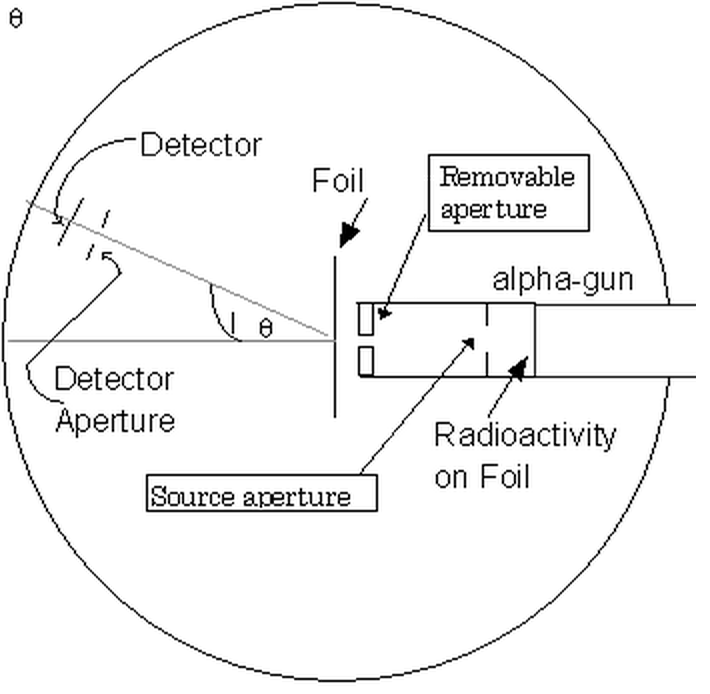
\includegraphics[width = 5 cm]{Diagram.png}
% %   \begin{center}
% %   \caption{Inside the vacuum chamber}[\footnotesize{``Rutherford Scattering.'' - Physics 111-Lab Wiki. UC Berkeley, n.d. Web. 13 Mar. 2015.}]
% %   \label{Diagram}
% %   \end{center}
% % \end{figure}

% % \begin{figure}[h]
% %   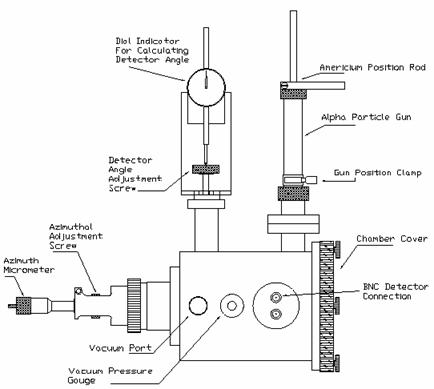
\includegraphics[width = 5 cm]{Diagram2.jpg}
% %   \begin{center}
% %   \caption{Outside the vacuum chamber}[\footnotesize{``Rutherford Scattering.'' - Physics 111-Lab Wiki. UC Berkeley, n.d. Web. 13 Mar. 2015.}]
% %   \label{OutisdeDiagram}
% %   \end{center}
% % \end{figure}

% \subsection{Taking Measurements}

% For our experiment, we first created a vacuum in the chamber. Then we adjusted the Tran-L-Amp to where we set the DIFF to 1.0, INT to 0.05, Coarse Gain to 100, Vennier Gain to  5.9 microseconds, and the FINE GAIN at 1.75. Finally, with the detector at 0 degrees, we make sure that the detector is receiving a signal that displays on the oscilloscope. An example of this signal is in Figure~\ref{Scope}.

% % \begin{figure}[h]
% %   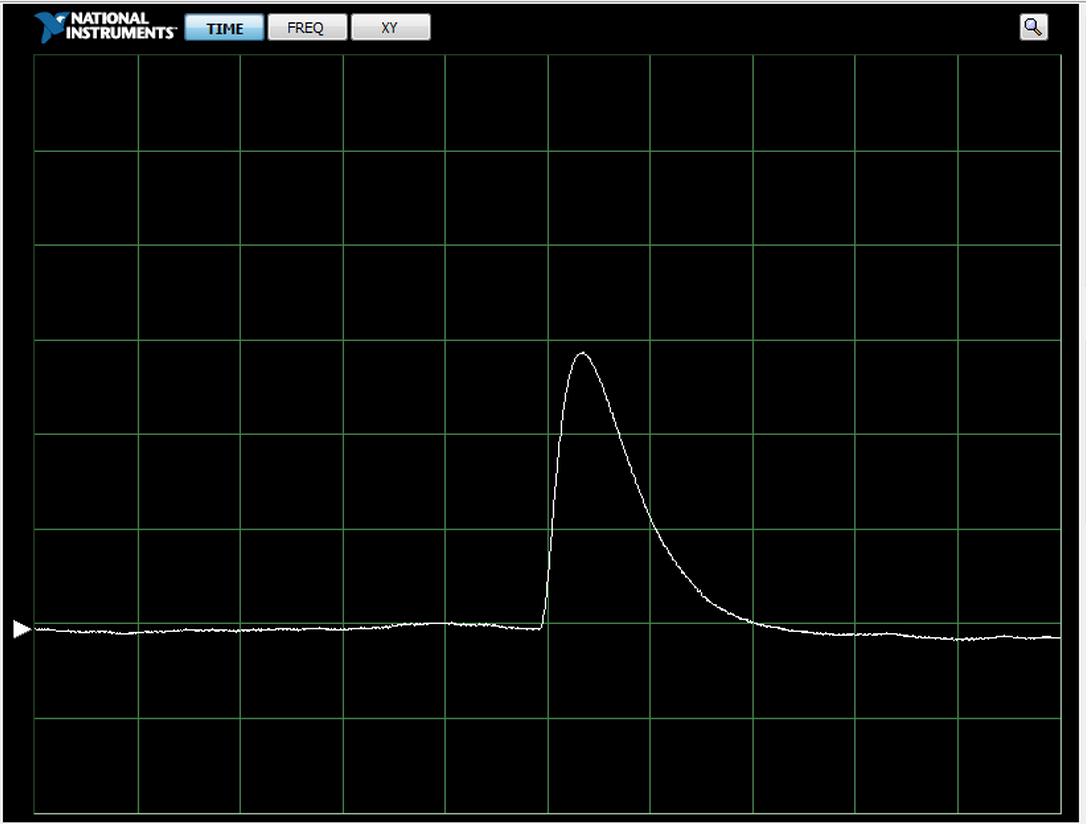
\includegraphics[width = 5 cm]{Scope.png}
% %   \begin{center}
% %   \caption{The feed into the scope}[\footnotesize{``Rutherford Scattering.'' - Physics 111-Lab Wiki. UC Berkeley, n.d. Web. 13 Mar. 2015.}]
% %   \label{Scope}
% %   \end{center}
% % \end{figure}

% \section{Measurements and Analysis}

% when we took measurements, we first took measurements of the intensity of the alpha gun itself, then the angle dependence of the alpha particles without any gold foil, and then finally we included the gold foil and found the angle dependence. 

% In Table~\ref{PointBlank} we see the counting rate of the gun at point blank. This is much greater than the maximum counting rate of gun at its default position of 7.8 cm. With that distance, the maximum counting rates were much less than the point blank counting rate. However, we can see from Table~\ref{NoFoilTable} that when the point rates of the angles are summed up, we get near the total counts when we have the gun at point blank. This indicates to us that the alpha particle beam is not emitting straight out of the gun; instead, it had an angular dependence. In the theory we discussed energy loss due to collisions with the walls of the gun. In Table~\ref{Energies}, however, we see that at an angle of 5 degrees, the mean energy is roughly the same for 0 degrees and point blank, and even the distribution in Figure~\ref{EnergiesGraph} looks similar. What is probably happening is that the alpha particle is colliding many times within the gun, and on average, alpha particles are colliding an equal amount of times before exiting the gun. Therefore, the average energy leaving the gun is angle independent. 

% We also noticed that in the case of no foil, the counts of alpha particles drops of very quickly past 5 and -5 degrees (see the left plot in Figure~\ref{Combined}). This means that when we insert the gold foil, counts that we receive past 10 and -10 degrees are most likely due to alpha particles scattering off the gold foil.

% \begin{table}[h]
% \begin{tabular}{|l|l|}
% \hline 
% Measurement & Count Rate (counts/s)                \\ \hline \hline
% Point Blank & 104.84 $\pm$ 10.39                        \\
% No Foil, 7.8 cm away from detector & 65.86 Max Value    \\
% With Foil, 7.8 cm away from detector & 40.76 Max Value  \\ \hline         
% \end{tabular}
% \label{PointBlank}
% \end{table}

% \begin{table}[h]
% \begin{tabular}{|l|l|}
% \hline
% No Foil Angle & Counting Rate (counts/s) \\ \hline \hline
% -5            & 4.70                          \\
% 0             & 65.86                         \\
% 2.5           & 32.96                         \\
% 5             & 22.54                         \\
% 7.5           & 3.863333333                   \\ \hline
% \end{tabular}
% \label{NoFoilTable}
% \end{table}

% \begin{table}[h]
% \begin{tabular}{|l|l|}
% \hline
% Angle (Degrees) with No Foil & Energy    \\ \hline \hline
% 0               & 4.75 $\pm$ 0.74        \\
% 5               & 4.74 $\pm$ 0.67        \\
% Point Blank     & 4.69 $\pm$ 0.94        \\ \hline
% \end{tabular}
% \label{Energies}
% \end{table}

% % \begin{figure}[h]
% %   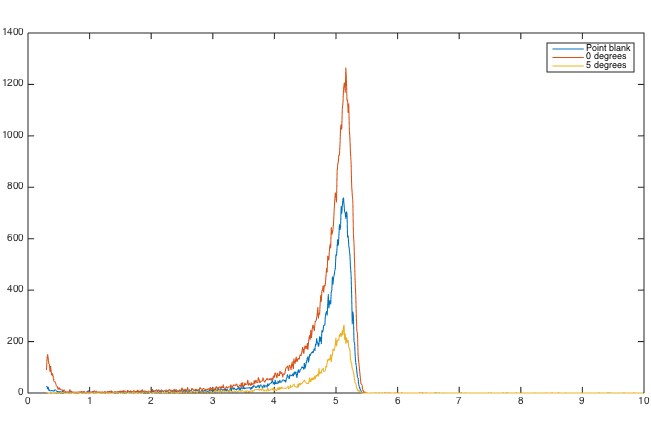
\includegraphics[width = 5 cm]{pointblankcomparison.png}
% %   \begin{center}
% %   \caption{Comparison between three configurations without foil.}
% %   \label{EnergiesGraph}
% %   \end{center}
% % \end{figure}


% % \begin{figure*}[t]
% %   \includegraphics[width=\textwidth]{Combined Graphs.png}
% %   \begin{center}
% %   \caption{Gaussian Fit of angle vs. counting rates for both no foil and with foil}
% %   \label{Combined}
% %   \end{center}
% % \end{figure*}

% Now that we've seen how the alpha particles scatter without the gold foil, we can begin looking at the scattering with the gold foil in place. We fit the data to a Gaussian Distribution because the data points looked like they were following a Gaussian curve. Figure~\ref{Combined} shows a wider distribution for the angle, which confirms our theory that gold can scatter alpha particles beyond small angles. For the case of the foil, the standard deviation is 3.94 degrees, which is 48\% larger than 2.66 degrees the standard deviation for no foil. Although there is a difference, this degree of difference is not unexpected, due to the tiny size of the gold nucleus, which is on the order of femtometers. We ought to be seeing a wider spread for the case of the gold foil, but not an absurdly large difference since the small size of the nucleus means that most alpha particles will be deflected a small amount. Large angle deflections would be indicative of alpha particles either coming very close (distance << the size of a gold atom) to one or multiple gold nuclei. 

% \begin{table}[h] 
%   \begin{tabular}{|l|l|l|}
%   \hline
%   Measurement & $\mu$ (Degrees) & $\sigma$ of Zero-Position \\ \hline \hline
%   No Foil     & 0.1401  (-3.03, 3.311) & 3.761  (0.3299, 7.192)     \\ 
%   With Foil   & -0.7366  (-2.407, 0.9333) & 5.568  (2.813, 8.322) \\ \hline     
%   \end{tabular}
%   \caption{Gaussian Fit of Counting Rate Data (with 95$\%$ confidence bounds)[\footnotesize{Note: Our plot with gold foil also shows an outlying point at 2.5 degrees and large 95$\%$ confidence intervals for the plot for no foil. We will discuss these discrepancies in the error section of our paper.}]}
%   \label{ZeroPosition}
% \end{table}

% \begin{table}[h] 
%   \begin{tabular}{|l|l|l|}
%   \hline
%   Measurement & $\mu$ (Degrees) & Magnitude of Peak (counts/s) \\ \hline \hline
%   No Foil     & 0.1401  (-3.03, 3.311) & 61.54  (17.1, 106)    \\ 
%   With Foil   & -0.7366  (-2.407, 0.9333) & 29.22  (18.98, 39.46)  \\ \hline     
%   \end{tabular}
%   \caption{Continuation of Table~\ref{ZeroPosition}
%   \label{ZeroPosition2}
% \end{table}

% Another observation that we made was that the counting rate with the gold foil is less than the counting rate for the case without gold foil. The maximum counting rate near the 0 angle position, according to the Gaussian Fit, was 30 fewer counts/second in the case of the gold foil. This difference is expected due to alpha particles getting scattered outwards from the 0 angle. 


% % \begin{figure*}[t]
% %   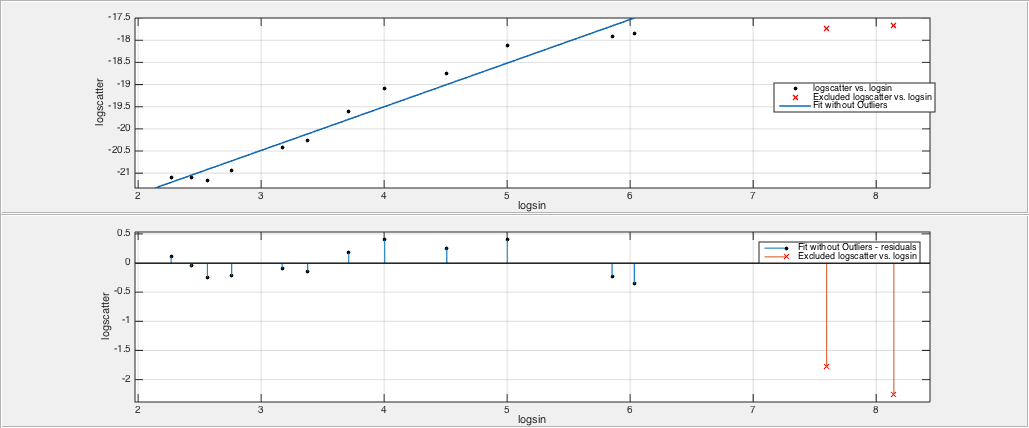
\includegraphics[width=\textwidth]{FitforScatteringCrossSection.png}
% %   \begin{center}
% %   \caption{Scattering Cross Section vs. $ \sin(\frac{\theta}{2}))^{-4}$}
% %   \label{FitforScatteringCrossSection}
% %   \end{center}
% % \end{figure*}

% With these plots, we can begin to calculate the atomic number of the gold atom. 

% \begin{table}[h]
%   \begin{tabular}{|l|l|}
%   \hline 
%   Variable                         & Value               \\ \hline \hline 
%   Incident Counting Rate           & 112.19 counts/sec   \\
%   Detector Solid Angle             & 0.0060 sr           \\
%   Area Density of Gold Foil        & $1.62 * 10^{21} atoms/cm^2$ \\
%   Atomic Number of Alpha Particle  & 2                   \\
%   Average Energy of Alpha Particle & 3.863333333        \\ \hline
%   \end{tabular}
%   \label{Values}
% \end{table}

% % \begin{figure}[h]
% %   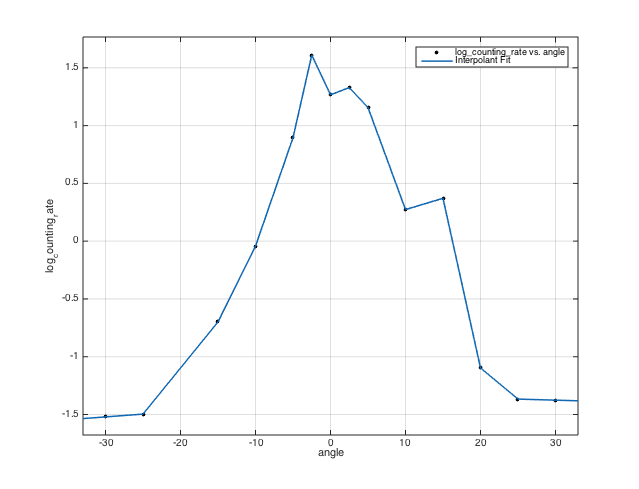
\includegraphics[width=5 cm]{InterpolantFit.png}
% %   \begin{center}
% %   \caption{Scattering Cross Section vs. $\sin(\theta))^{-4}$}
% %   \label{InterpolantFit}
% %   \end{center}
% % \end{figure}

% % \begin{figure}[t]
% %   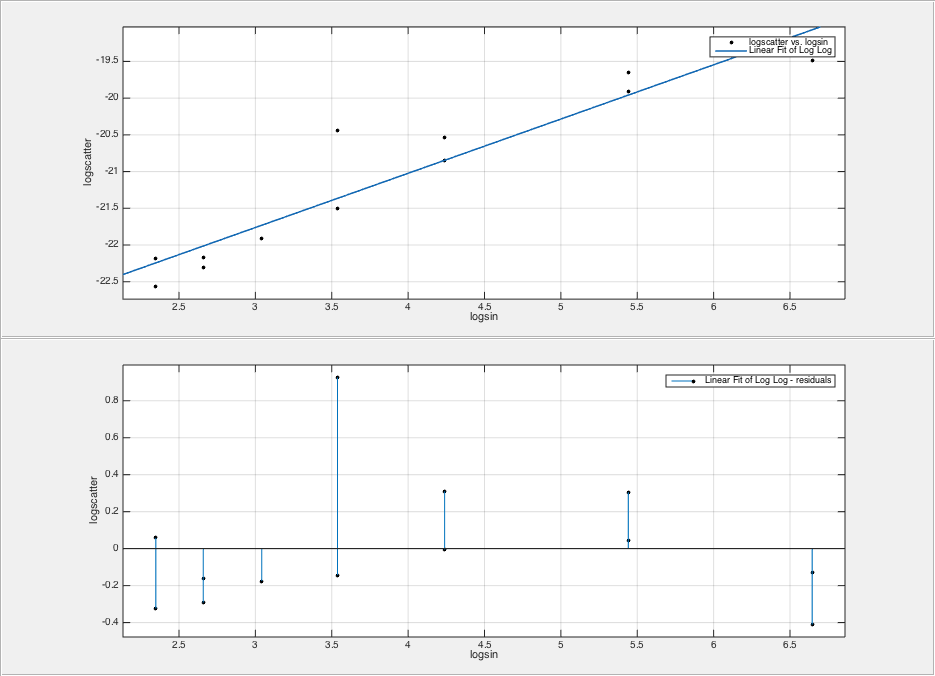
\includegraphics[width = 5 cm]{LinearFitLogLog.png}
% %   \begin{center}
% %   \caption{Outside the vacuum chamber}
% %   \label{OutisdeDiagram}
% %   \end{center}
% % \end{figure}

% % \begin{figure}[t]
% %   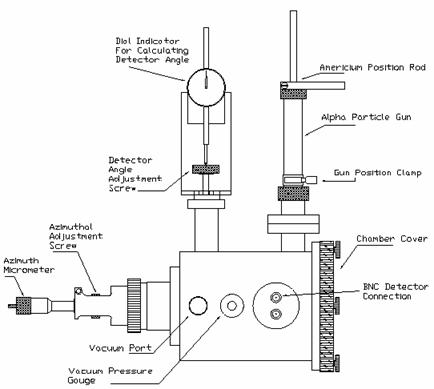
\includegraphics[width = 5 cm]{Diagram2.jpg}
% %   \begin{center}
% %   \caption{Outside the vacuum chamber}
% %   \label{OutisdeDiagram}
% %   \end{center}
% % \end{figure}


% \subsection{Longitudinal Electric Field without a Magnetic Field} 


% \subsection{Magnetic Field Strength}


% \subsection{The Hall Effect}


% \section{Error Discussion}

% % \begin{figure}[h]
% %   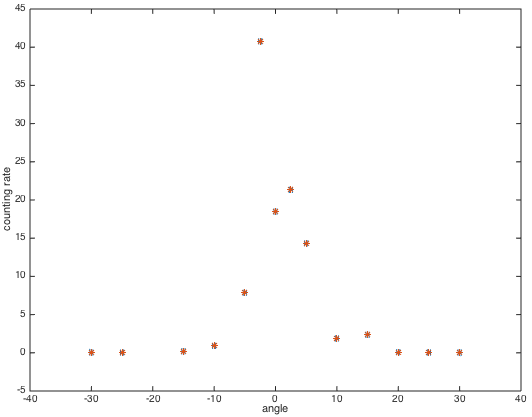
\includegraphics[width=5 cm]{errorfoil.png}
% %   \begin{center}
% %   \caption{Error in Angle with Foil}
% %   \label{ErrorFoil}
% %   \end{center}
% % \end{figure}

% % \begin{figure}[h]
% %   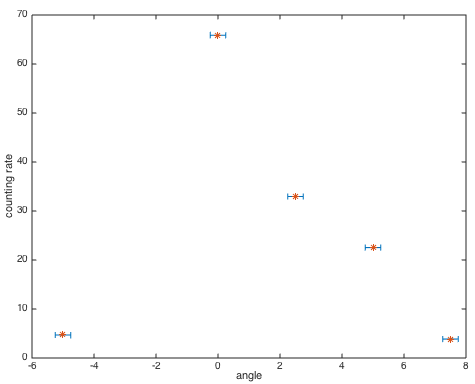
\includegraphics[width=5 cm]{errornofoil.png}
% %   \begin{center}
% %   \caption{Error in Angle without Foil}
% %   \label{ErrorNoFoil}
% %   \end{center}
% % \end{figure}

% \subsection{Collision Frequency}


% \subsection{Electron Drift Velocity and Number Density}



% \subsection{Electron Temperature}



% \section{Conclusion}



% %%%%%%%%%%%%%%%%%%%%%%%%%%%%%%%%%%%%%%%%%%%%%%%%%%%%%%%%%%%%%%%%%%%%%%%%%
% % Place all of the references you used to write this paper in a file
% % with the same name as following the \bibliography command
% %%%%%%%%%%%%%%%%%%%%%%%%%%%%%%%%%%%%%%%%%%%%%%%%%%%%%%%%%%%%%%%%%%%%%%%%%


% % %%%%%%%%%%%%%%%%%%%%%%%%%%%%%%%%%%%%%%%%%%%%%%%%%%%%%%%%%%%%%%%%%%%%%%%%%%%%%
% \begin{acknowledgments} I acknowledge my lab partner Tanooj Shah for taking data with me and helping me understand the pre-lab questions. I also want to acknowledge Prof Stamper-Kurn for asking challenging questions but ultimately pushing Tanooj and me to truly understand the lab.
% \end{acknowledgments}

% \begin{thebibliography}{9}

% \bibitem{Melissinos}
%   A.C. Melissinos, \emph{Experiments in Modern Physics}, Rutherford Scattering, Academic Press Inc. pg. 231-252, 1966

% \bibitem{youtube}
%   Sumner Davis, \emph{Hall Effect in Plasma}, http://youtu.be/iZkOlZDyb2U, March 7, 2012

% \bibitem{Kunkel}
%   W. B. Kunkel, \emph{Hall Effect in a Plasma}, American Journal of Physics, Number 733, Volume 49, 1981

% \bibitem{website}
%   Physics 111 ADV Lab, \emph{Hall Effect in a Plasma}, http://advancedlab.berkeley.edu/, February, 2015

% \bibitem{Comfort}
% J.R. Comfort, et al., \emph{Energy Loss and Straggling of α Particles in Metal Foils}, Phys. Rev. 150, 249 (1966)

% \end{thebibliography}


\end{document}
